\subsection{Choose, justify and freeze the filter parameters}
\label{sec:r22}
I freeze $\RttLength $ symmetric \RttWindow{} taps, nominal half-width
$\RttHalfWidth $ Hz, delay $\RttDelay $ samples ($\RttDelayMs $ ms) and
$K=\RttFFT$, using the measured spectrum and rule below.

\paragraph{Corrupted-spectrum evidence.}
Spectral analysis of anchor phase-0 repeat 0 uses rectangular, symmetric
Hann and Hamming observation windows, distinct from FIR tapers. Equations~\eqref{eq:r22-spectrum-scales}
and \eqref{eq:r22-psd-integral} set amplitude/PSD scales and Parseval.
Native PSD uses $K=N$; literal $-3.000$ dB amplitude widths use 16-fold
padding and interpolated crossings:
\begin{align}
 \widehat S_{\rm bg}&=\frac1{|\mathcal B|}
       \sum_{k\in\mathcal B}\widehat S_{{\rm rect},N}[k],&
 L_i&=10\log_{10}\frac{\widehat S_{{\rm rect},N}[k_i]}
                            {\widehat S_{\rm bg}},\nonumber\\
 A_{\rm threshold}&=A_{\rm local\,peak}10^{-3/20},&
 W_{-3{\rm dB}}&=f_R-f_L.
 \label{eq:r22-spectrum-measures}
\end{align}
$\mathcal B $ comprises interior positive bins outside $\pm20 $ Hz of
the four priors. The mean off-band PSD is $\RttPsdBackground $ squared
NPY units/Hz; the 6 kHz peak lies $\RttWeakPeakBackground $ dB above it.
Padding refines the grid to 0.03125 Hz, not the 0.5 Hz native resolution;
power/amplitude ratios use 10/20 log, respectively.

\begin{table}[!htbp]
 \centering\small
 \caption{Corrupted-spectrum evidence. Analysis-peak widths are Hz, distinct from FIR passbands; peak/background uses native rectangular PSD.}
 \label{tab:r22-spectrum}
 \begin{tabular}{rrrrr}
\toprule
Centre (Hz) & Peak/background (dB) & Rect. width & Hann width & Hamming width \\
\midrule
440 & 43.00 & 0.4414 & 0.7185 & 0.6496 \\
1320 & 38.71 & 0.4400 & 0.7103 & 0.6432 \\
2200 & 32.68 & 0.4432 & 0.7240 & 0.6546 \\
6000 & 23.46 & 0.4353 & 0.7207 & 0.6475 \\
\bottomrule
\end{tabular}

\end{table}


\begin{figure}[!htbp]
 \centering
 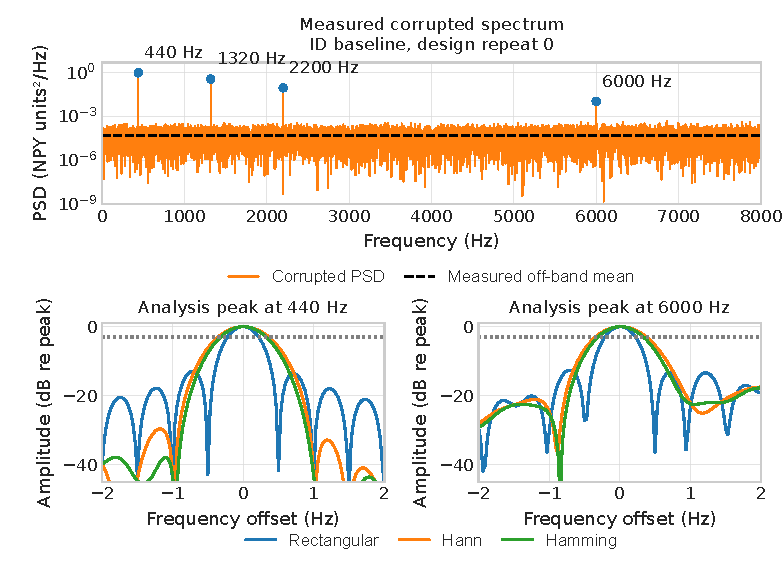
\includegraphics[width=.82\linewidth]{supporting/publication_r22_corrupted_spectral_evidence.pdf}
 \caption{Personal phase-0 spectrum: native PSD/background above; three observation-window peaks and interpolated $-3.000$ dB widths below.}
 \label{fig:r22-corrupted-evidence}
\end{figure}

Sub-hertz observation widths support separated bands; finite-FIR
passbands also depend on truncation, gain and boundaries.
\paragraph{Measured search with explicit constraints.}
The project-designed kernel uses the reference window formulas in
Eqs.~\eqref{eq:r22-family} and \eqref{eq:r22-windows}.
Six lengths 129/257/513/1025/2049/4097, seven half-widths
2/5/10/20/40/80/160 Hz and three tapers give 126 coarse candidates.
Require positive aligned gain within 1\% over centre $\pm2$ Hz,
checked every 0.5 Hz:
\begin{equation}
 G(f)=\sum_{m=0}^{M-1}h[m]e^{-j2\pi f(m-d)/f_s},\qquad
 \bigl||G(f_i+\delta)|-1\bigr|\le0.01.
 \label{eq:r22-gain-constraint}
\end{equation}
The guard is a design allowance, not measured drift. All candidates share
18 design records; selection uses $\mathcal C=\{0,10,20,30,S_0\}$ dB,
$R=3$, and the balanced score
\begin{equation}
 J=\frac1{|\mathcal C|R}\sum_{c\in\mathcal C}\sum_{r=0}^{R-1}
 \frac{\mathrm{MSE}_{\rm out}(c,r)}{\mathrm{MSE}_{\rm in}(c,r)}.
 \label{eq:r22-objective}
\end{equation}
Each MSE includes 32000 samples; paired normalisation balances SNRs.
The $-10$ dB stress point is excluded. Reference-based scoring supplies no
truth to recovery. Refining adjacent bounds around the feasible minimum
uses seven odd lengths and 13 widths rounded to 0.5 Hz; with coarse
points, $\RttCount$ candidates include $\RttFeasible$ feasible choices.
Within 1\% of minimum $J$, prefer shortest length, then lower $J$,
narrower band and registered window order. The winner is also the strict
tested minimum and is unchanged at 0/0.5/1\% allowances.

\begin{figure}[!htbp]
 \centering
 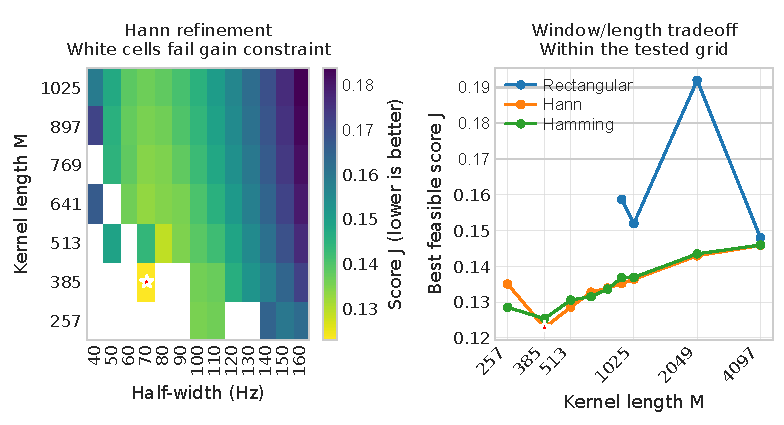
\includegraphics[width=.82\linewidth]{supporting/publication_r22_parameter_search.pdf}
 \caption{Hann refinement (white: gain-guard failure) and each taper's best feasible tested width at each length. Star: frozen 385-tap choice.}
 \label{fig:r22-search}
\end{figure}


\begin{table}[!htbp]
 \centering\small
 \caption{Best feasible tested candidate per kernel taper. Scores use the same declared paired design objective, not a universal window ranking.}
 \label{tab:r22-windows}
 \begin{tabular}{lrrrr}
\toprule
Kernel window & $M$ & Half-width (Hz) & $J$ & Clean-input MSE \\
\midrule
Rectangular & 4097 & 80 & 0.147986 & $2.2352\times10^{-4}$ \\
Hann & 385 & 70 & 0.122854 & $2.2951\times10^{-4}$ \\
Hamming & 385 & 70 & 0.125388 & $2.3551\times10^{-4}$ \\
\bottomrule
\end{tabular}

\end{table}

\paragraph{Result, reason and cost.}
The four nominal positive bands are
 $[370,510]$, $[1250,1390]$, $[2130,2270]$ and $[5930,6070]$
 Hz, plus conjugate negative bands.
Realised $-3 $ dB full widths are about $\RttBandWidthMin $ Hz; they are not
the 140 Hz template widths. Maximum guard gain deviation is
$\RttGainPercent $\%. Relative to the 513-tap prototype, score falls from
$\RttOldScore $ to $\RttScore $ ($\RttScoreImprovement $\%), and group delay
from 16 to 12 ms. Both use the same FFT length; runtime gain is unmeasured.
Whole-record buffering is 2 s, so group delay is not total latency. Clean MSE rises to $\RttCleanMse $,
while finite-record noise gain falls to $\RttNoiseGain $; at 30 dB design
MSE $\RttHighNew $ exceeds the prototype's $\RttHighOld $.

\begin{figure}[!htbp]
 \centering
 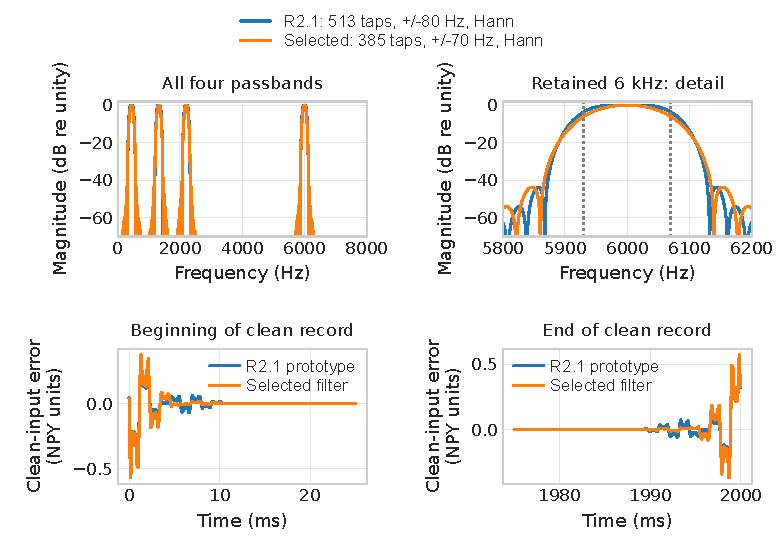
\includegraphics[width=.82\linewidth]{supporting/publication_r22_response_boundary.pdf}
 \caption{Realised FIR response and retained clean-input endpoint distortion. Template edges and measured $-3.000$ dB widths differ.}
 \label{fig:r22-response-boundary}
\end{figure}

The fixed-filter expectation $ D+\sigma^2G_{\rm finite}$ predicts a
sample-grid crossover near $\RttCrossover $ dB (Appendix~\ref{app:filter});
every trial retains its cross term. Ten checks cover PSD, IDFT,
convolution, symmetry and finite-boundary gain. Coefficients/hashes in
\path{stage2/r22/results/filter_freeze.json} precede phase 1.
